%% 국문 번역본 (저자 참고용). 영문 원고의 번역이다.
\documentclass[11pt,a4paper]{article}
\usepackage[top=25mm,bottom=25mm,left=25mm,right=25mm]{geometry}
\usepackage{fontspec}
\setmainfont{Nanum Myeongjo}
\XeTeXlinebreaklocale "ko"
\XeTeXlinebreakskip=0pt plus 1pt minus .5pt
\usepackage{amsmath,amssymb,amsthm,mathtools}
\usepackage{tikz}
\usepackage[hidelinks]{hyperref}
\hypersetup{colorlinks=true,linkcolor=black,citecolor=black,urlcolor=blue}
\linespread{1.25}
\setlength{\parindent}{1em}
\setlength{\emergencystretch}{3em}
\theoremstyle{definition}
\newtheorem{theorem}{정리}[section]
\newtheorem{lemma}[theorem]{보조정리}
\newtheorem{proposition}[theorem]{명제}
\newtheorem{corollary}[theorem]{따름정리}
\newtheorem{remark}[theorem]{비고}
\newtheorem{question}[theorem]{질문}
\newtheorem{problem}[theorem]{문제}
\renewcommand{\proofname}{증명}
\renewcommand{\refname}{참고문헌}
\renewcommand{\abstractname}{초록}
\renewcommand{\figurename}{그림}
\renewcommand{\tablename}{표}
\newcommand{\Dom}{\mathcal{D}}
\newcommand{\Crit}{\operatorname{Crit}}
\DeclareUrlCommand\lean{\urlstyle{tt}\def\UrlBreaks{\do\_}}
\newcommand{\MaxLC}{26}
\newcommand{\MinNonLC}{27}
\newcommand{\MaxOrder}{27}
\newcommand{\TotalTreesLC}{447\,672\,596}
\newcommand{\TotalTreesAll}{1\,198\,738\,056}
\newcommand{\MaxJumpValue}{1.04}
\newcommand{\AuthorEmail}{skdl3965@gmail.com}


\title{\textbf{상지배 간격이 4 이하인 숲의 지배다항식의 단봉성}\thanks{이 문서는 영문 원고
\emph{Unimodality of domination polynomials of forests with upper domination gap at most four}의
국문 번역본이며, 저자 참고용이다. 학술지 투고본은 영문 원고이다.}}
\author{홍찬우\\ {\normalsize 경인교육대학교}\\ {\normalsize \texttt{\AuthorEmail}}}
\date{}

\begin{document}
\maketitle

\begin{abstract}
그래프 $G$의 지배수를 $\gamma(G)$, 상지배수를 $\Gamma(G)$라 하자. Beaton과
Schoonhoven(2024)은 $\Gamma(T)-\gamma(T)\le2$인 나무 $T$의 지배다항식이 단봉임을
증명하였다. 이 논문에서는 $\Gamma(F)-\gamma(F)\le4$인 모든 숲 $F$의 지배다항식이
단봉임을 증명한다. 더 일반적으로, 고립점이 없는 위수 $n$의 숲에서 지배다항식이 단봉이
아니라면 $h=\Gamma(F)-\gamma(F)$에 대해 $n\le6\lceil(h+1)^2/4\rceil-h-16$이 성립한다.
특히 그러한 숲에서 $h\le\sqrt{2n/3}-1$이면 지배다항식은 단봉이다. 증명은 두 가지에
기초한다. 하나는 이분그래프 $G$의 지배집합 $S$가 가지는 임계 꼭짓점이
$2\alpha(G)-|S|$개 이하임을 보이는 짧은 논법이고, 다른 하나는 크기 $j$인 지배집합들의
평균 임계 꼭짓점 수가, $j-\gamma(F)\ge\lceil(h+1)^2/4\rceil$인 범위에서는 $j$가 1 늘 때 2보다 많이
늘 수 없음을 보이는 분산 평가이다.
$\Gamma-\gamma=4$인 경우에는 전수 계산이 추가로 쓰인다. 이 계산에 따르면 꼭짓점이
$\MaxLC$개 이하인 모든 나무의 지배다항식은 로그오목이고, 꼭짓점이 $\MinNonLC$개인 나무
가운데 로그오목이 아닌 것은 정확히 하나이다. 해석적 논증의 주요 단계는 Lean~4로
형식화하였다.

\medskip
\noindent\textbf{주제어.} 지배다항식, 단봉성, 로그오목성, 상지배수, 숲, 이분그래프

\noindent\textbf{2020 수학 주제 분류.} 05C69, 05C31, 05C05
\end{abstract}

\section{서론}\label{sec:intro}

이 논문에서 다루는 그래프는 모두 유한 단순 그래프이다. 그래프 $G$의 꼭짓점 집합
$S$가 \textbf{지배집합}이라는 것은 $S$ 밖의 모든 꼭짓점이 $S$ 안에 이웃을 가진다는
뜻이다. 크기가 $j$인 지배집합의 수를 $d_j(G)$라 할 때, 위수가 $n$인 그래프 $G$의
\textbf{지배다항식}은
\[
  D(G,x)=\sum_{j=0}^{n} d_j(G)\,x^j
\]
이다. 음이 아닌 수로 이루어진 수열 $(d_0,\dots,d_n)$이 어떤 $m$에 대하여
$d_0\le d_1\le\dots\le d_m\ge d_{m+1}\ge\dots\ge d_n$을 만족하면 \textbf{단봉}이라
하고, $1\le j\le n-1$에 대하여 $d_j^2\ge d_{j-1}d_{j+1}$을 만족하면
\textbf{로그오목}이라 한다. 다항식의 계수열이 이 성질을 가지면 그 다항식을 단봉 또는
로그오목이라 부른다. Alikhani와 Peng~\cite{AP}은 모든 그래프의 지배다항식이 단봉이라고
추측하였다. 이 추측은 나무에 대해서도 풀리지 않았다.

지금까지 알려진 결과는 \cite{BB22,BO,BS,DHP,GZ,Omar}에서 찾아볼 수 있다. Beaton과
Brown~\cite{BB22}은 최소 차수가 충분히 큰 그래프에 대해 단봉성을 증명하였고,
지배다항식이 로그오목이 아닌 9개 꼭짓점의 그래프를 제시하였다. Burcroff와
O'Brien~\cite{BO}은 $D(G,x)$의 계수가 대략 $(n+\Gamma(G))/2$ 이후로 증가하지 않음을
보였다. 여기서 \textbf{상지배수} $\Gamma(G)$는 극소 지배집합의 최대 크기이다. 나무에
대해서는 Beaton과 Schoonhoven~\cite{BS}이 지배다항식이 로그오목이 아닌 무한 족을
구성하였고, $\gamma$가 지배수일 때 $\Gamma(T)-\gamma(T)<3$인 모든 나무 $T$에 대해
$D(T,x)$가 단봉임을 증명하였다. 이 논문에서는 $\Gamma(G)-\gamma(G)$를 $G$의
\textbf{상지배 간격}이라 부른다. 간격이 0인 그래프는 잘 지배되는(well-dominated)
그래프이다.

이 논문의 목적은 Beaton과 Schoonhoven의 결과를 세 방향으로 확장하는 것이다. 나무에서
숲으로, 간격 2 이하에서 간격 4 이하로, 그리고 고정된 간격에서 위수와 함께 커질 수
있는 간격으로 확장한다.

\begin{theorem}\label{thm:gapfour-intro}
숲 $F$가 $\Gamma(F)-\gamma(F)\le 4$를 만족하면 $F$의 지배다항식은 단봉이다.
\end{theorem}

간격이 더 큰 경우에는, 주어진 간격마다 유한 개를 제외한 모든 숲에 대해 단봉성을
얻는다. 고립점은 지배다항식에 $x$의 거듭제곱을 곱할 뿐이므로 따로 다룬다.

\begin{theorem}\label{thm:criterion-intro}
$F$를 위수 $n$인 숲이라 하고 $h=\Gamma(F)-\gamma(F)$,
$K_h=\lceil (h+1)^2/4\rceil$이라 하자.
\begin{enumerate}
\item[\textup{(i)}] $n-\gamma(F)\ge 3K_h-7$이면 $D(F,x)$는 단봉이다.
\item[\textup{(ii)}] $F$에 고립점이 없고 $D(F,x)$가 단봉이 아니면 $h\ge 3$이고
$n\le 6K_h-h-16$이다.
\item[\textup{(iii)}] 특히 $F$에 고립점이 없고 $3h^2+4h-19\le 2n$이면 $D(F,x)$는
단봉이다.
\end{enumerate}
\end{theorem}

예를 들어 $\Gamma(F)-\gamma(F)\le\sqrt{2n/3}-1$이면 (iii)을 적용할 수 있다. (ii)의
상계는 $h=3$일 때 $5$, $h=4$일 때 $22$, $h=5$일 때 $33$이다. 정리~\ref{thm:gapfour-intro}의
$h=3$인 경우는 여기서 별 그래프 $K_{1,4}$ 하나만 살펴보면 따라 나온다. $h=4$인
경우에는 꼭짓점이 $22$개 이하인 숲의 지배다항식이 필요하며, 이를 위해 계산에
의존한다. 이 계산은 필요한 것보다 더 많은 사실을 확립하며 그 자체로도 의미가 있다.

\begin{theorem}\label{thm:smalltrees-intro}
\begin{enumerate}
\item[\textup{(i)}] 꼭짓점이 $\MaxLC$개 이하인 모든 나무의 지배다항식은 로그오목이다.
따라서 모든 성분의 꼭짓점이 $\MaxLC$개 이하인 숲의 지배다항식은 로그오목이며, 특히
단봉이다.
\item[\textup{(ii)}] 꼭짓점이 $\MinNonLC$개인 나무 $751\,065\,460$개 가운데 지배다항식이
로그오목이 아닌 것은 정확히 하나이다.
\end{enumerate}
\end{theorem}

예외가 되는 나무는 그림~\ref{fig:U}에 있으며, 그 지배다항식은 단봉이다. 따라서
지배다항식이 로그오목이 아닌 나무의 최소 위수는 $\MinNonLC$이다. Beaton과
Schoonhoven~\cite{BS}의 나무는 꼭짓점이 $9k+4$개이고, 그 논문에서는 $k\ge4$일 때, 즉
위수 $40$부터 로그오목이 아님을 보였다. 최근 \cite{DHP}에서는 기계학습 소프트웨어
PatternBoost를 사용하여 지배다항식이 로그오목이 아닌 나무와 그래프를 더 찾았는데,
그 논문에 제시된 나무는 꼭짓점이 $32$개와 $58$개이다. 같은 논문은 지배다항식의
로그오목성이 임의로 많은 지표에서 깨지는 나무도 구성한다. 최소 위수가
$\MinNonLC$이라는 사실은 독립다항식의 경우와 닮았다. Kadrawi와 Levit~\cite{KL}은
나무의 독립다항식에서 로그오목성이 위수 $26$에서 처음 깨짐을 발견하였다.

\subsection*{방법}
지배집합 $S$의 꼭짓점 $v\in S$는 $S\setminus\{v\}$가 지배집합이 아닐 때
\textbf{임계}라고 하고, $S$의 임계 꼭짓점의 수를 $a(S)$로 쓴다. 크기가 연속한 두
지배집합의 포함 쌍을 세면, $d_{j-1}\le d_j$는 크기 $j$인 지배집합들에서 $a(S)$의
평균이 $2j-n-1$ 이상이라는 것과 동치임을 알 수 있다. 이 관찰이 \cite{BS}의 출발점이다.
Beaton과 Schoonhoven은 나무 $T$의 모든 지배집합 $S$가
\begin{equation}\label{eq:BS-bounds}
  2\gamma(T)-|S|\;\le\; a(S)\;\le\; 2\Gamma(T)-|S|
\end{equation}
를 만족함을 증명하고, 이로부터 계수가 대략 $(n+2\gamma)/3$까지 증가하고 대략
$(n+2\Gamma)/3$부터 감소함을 이끌어 냈다. $\Gamma-\gamma\le2$이면 결정되지 않는
단계가 많아야 하나 남는다.

이 논문의 기여는 두 부분이다. 첫째, \eqref{eq:BS-bounds}의 상계에 대한 짧은 증명을
제시한다. 이 증명은 모든 이분그래프에 적용되며 부등식
$|S|+a(S)\le 2\alpha(G)$를 준다(보조정리~\ref{lem:upper}). 여기서 $\alpha$는
독립수이다. \cite{BS}에 있는 나무에 대한 원래 증명은 길고 재구성 논법에 의존한다.
부산물로, \cite{BS}의 감소 구간과 지배집합 평균 크기의 상계가 모든 이분그래프로
확장된다(따름정리~\ref{cor:segments}). 둘째, 더 중요하게는, 두 단조 구간 사이에 남는
창을 제어한다. 크기 $j$인 지배집합들에서 $a(S)$의 평균을 $c_j$라 하면,
\textbf{골짜기} $d_{i-1}\ge d_i<d_{i+1}$는 $c_{i+1}-c_i>2$를 강제한다
(보조정리~\ref{lem:valley}). 한편 연속한 두 계급 사이의 공분산 부등식을
\eqref{eq:BS-bounds} 및 초등적인 분산 상계와 결합하면
$j-\gamma\ge\lceil (h+1)^2/4\rceil$일 때 $c_{j}-c_{j-1}\le 2$를 얻는다
(보조정리~\ref{lem:jump}). 위수가 간격에 비해 크면 이 범위가 창 전체를 덮는다. 여기서
$j$에 대한 제한은 필요하다. 모든 숲에서 $c_{j+1}-c_j<2(j-\gamma)+1$이 성립하고 이
상계가 나무에서 최선임을 보이는데, 따라서 차 $c_{j+1}-c_j$는 $2$를 넘을 수 있고 실제로
유계가 아니다(명제~\ref{prop:jumps}).

\subsection*{검증}
간격 4에 대한 정리~\ref{thm:gapfour-intro}와 정리~\ref{thm:smalltrees-intro}는 전수
계산에 의존한다. 이 계산은 서로 다른 나무 생성 알고리즘과 같은 지배다항식 점화식의 동치 형태를 별도로 구현한 두
프로그램으로 수행하였다(부록~\ref{app:computation}). 또한 해석적 논증의 주요 명제를
Mathlib을 사용하는 Lean~4~\cite{Lean,Mathlib}로 형식화하였다. 형식화의 정확한 범위는
부록~\ref{app:lean}에 기술한다. 프로그램, 그 출력, Lean 소스는 보충자료로 이 논문에
첨부한다.

\subsection*{구성}
\ref{sec:prelim}절에서는 기본 사실을 모은다. \ref{sec:critical}절에서는 $a(S)$에 대한
두 부등식과 그 직접적인 귀결을 다룬다. \ref{sec:jump}절에서는 평균 $c_j$를 연구하고,
\ref{sec:unimodal}절에서는 정리~\ref{thm:criterion-intro}와
정리~\ref{thm:gapfour-intro}의 간격 3 이하인 경우를 증명한다. \ref{sec:small}절에서는
작은 나무를 다루고 정리~\ref{thm:gapfour-intro}의 증명을 마친다.
\ref{sec:remarks}절에는 비고와 질문을 싣는다.

\section{준비}\label{sec:prelim}

$G$를 꼭짓점 집합이 $V$이고 위수가 $n=|V|$인 그래프라 하자. $v\in V$의 닫힌 근방을
$N[v]$로 쓴다. 그러면 $S\subseteq V$가 지배집합일 필요충분조건은 모든 $u\in V$에 대해
$N[u]\cap S\ne\emptyset$인 것이다. 지배집합의 어떤 진부분집합도 지배집합이 아니면
그 지배집합을 \textbf{극소}라고 한다. 지배집합의 최소 크기를 $\gamma(G)$, 극소
지배집합의 최대 크기를 $\Gamma(G)$, 독립집합의 최대 크기를 $\alpha(G)$로 쓴다.
크기가 $j$인 지배집합의 족을 $\Dom_j(G)$라 하면 $d_j=d_j(G)=|\Dom_j(G)|$이다.
$j<0$이거나 $j>n$이면 $d_j=0$으로 둔다.

지배집합 $S$에 대하여
\[
  \Crit(S)=\{v\in S:\ S\setminus\{v\}\text{는 지배집합이 아니다}\},\qquad
  a(S)=|\Crit(S)|
\]
라 하자. 꼭짓점 $v\in S$가 임계일 필요충분조건은 \textbf{사적 증인}, 즉
$N[u]\cap S=\{v\}$인 꼭짓점 $u$가 존재하는 것이다. 지배집합 $S$가 극소일 필요충분조건은
$a(S)=|S|$이다.

\begin{lemma}\label{lem:basic}
$G$를 위수 $n$인 그래프라 하자.
\begin{enumerate}
\item[\textup{(i)}] $d_j>0$일 필요충분조건은 $\gamma(G)\le j\le n$이다.
\item[\textup{(ii)}] $S\subseteq U$가 지배집합이면 $\Crit(U)\subseteq\Crit(S)$이다.
\item[\textup{(iii)}] $1\le j\le n$에 대하여
\begin{equation}\label{eq:incidence}
  (n-j+1)\,d_{j-1}=\sum_{S\in\Dom_j(G)}\bigl(j-a(S)\bigr).
\end{equation}
\end{enumerate}
\end{lemma}

\begin{proof}
(i) 지배집합을 포함하는 집합은 모두 지배집합이다.

(ii) $v\in\Crit(U)$라 하자. $v\notin S$이면 $S\subseteq U\setminus\{v\}$이므로
$U\setminus\{v\}$가 지배집합이 되어 모순이다. 따라서 $v\in S$이고,
$S\setminus\{v\}\subseteq U\setminus\{v\}$는 지배집합이 아니다.

(iii) $S'\in\Dom_{j-1}(G)$, $S\in\Dom_j(G)$, $S'\subset S$인 쌍 $(S',S)$를 센다. 각
$S'$는 정확히 $n-j+1$개의 $S$로 확장되고, 각 $S$는 크기 $j-1$인 지배 부분집합을
정확히 $j-a(S)$개 포함한다.
\end{proof}

다음 두 사실은 잘 알려져 있다. 짧은 증명을 함께 싣는다.

\begin{lemma}[Ore~\cite{Ore}]\label{lem:ore}
$G$를 고립점이 없는 위수 $n$의 그래프라 하자. $G$의 모든 극소 지배집합의 여집합은
지배집합이다. 특히 $n\ge\gamma(G)+\Gamma(G)$이다.
\end{lemma}

\begin{proof}
$M$을 극소 지배집합, $v\in M$, $u$를 $v$의 사적 증인이라 하자. $u\ne v$이면
$u\notin M$이므로(그렇지 않으면 $N[u]\cap M\supseteq\{u,v\}$) $v$는 $M$ 밖에 이웃을
가진다. $u=v$이면 $v$는 $M$ 안에 이웃이 없고, 고립점이 아니므로 $M$ 밖에 이웃을
가진다. 따라서 $V\setminus M$은 $M$의 모든 꼭짓점을 지배한다. $|M|=\Gamma(G)$로
잡으면 $\gamma(G)\le n-\Gamma(G)$를 얻는다.
\end{proof}

\begin{lemma}\label{lem:isolates}
$G$를 고립점이 정확히 $r$개인 그래프라 하고, $G$에서 고립점을 모두 지운 그래프를
$G^{\circ}$라 하자. 그러면
\[
  D(G,x)=x^{r}D(G^{\circ},x),\qquad \gamma(G)=\gamma(G^{\circ})+r,\qquad
  \Gamma(G)=\Gamma(G^{\circ})+r
\]
이다. 특히 $G$와 $G^{\circ}$는 상지배 간격이 같고 $|V|-\gamma$의 값이 같으며,
$D(G,x)$가 단봉일 필요충분조건은 $D(G^{\circ},x)$가 단봉인 것이다.
\end{lemma}

\begin{proof}
$G$의 모든 지배집합은 고립점을 전부 포함한다. 고립점을 지우는 것은 $G$의 지배집합과
$G^{\circ}$의 지배집합 사이의 일대일 대응이며, 크기를 $r$만큼 줄이고 극소성을
보존한다.
\end{proof}

\section{숲과 이분그래프의 임계 꼭짓점}\label{sec:critical}

첫 번째 부등식은 나무에 대해 Beaton과 Schoonhoven~\cite[Lemma~5]{BS}이 얻은 것이다.
여기서는 자체로 완결된 증명을 제시한다. 가장 깊은 비임계 꼭짓점을 지운다는 그들의
생각을 따르며, 숲에 그대로 적용된다.

\begin{lemma}\label{lem:lower}
$S$가 숲 $F$의 지배집합이면 $|S|+a(S)\ge 2\gamma(F)$이다.
\end{lemma}

\begin{proof}
$|S|$에 대한 귀납법을 쓴다. $S$의 모든 꼭짓점이 임계이면
$|S|+a(S)=2|S|\ge2\gamma(F)$이다. $|S|=\gamma(F)$인 경우가 여기에 포함된다. 이제
$S\setminus\Crit(S)\ne\emptyset$이라 가정하자. $F$의 각 성분에서 꼭짓점 하나를 뿌리로
잡고, 꼭짓점의 깊이를 자기 성분의 뿌리까지의 거리로 정의한 뒤, 깊이가 최대인
$v\in S\setminus\Crit(S)$를 고른다. 집합 $S'=S\setminus\{v\}$는 지배집합이다. 다음을
주장한다.
\begin{equation}\label{eq:one-more}
  a(S')\le a(S)+1 .
\end{equation}
그러면 $|S'|+a(S')\le|S|+a(S)$이므로 $S'$에 귀납 가정을 적용하면 증명이 끝난다.

보조정리~\ref{lem:basic}(ii)에 의해 $\Crit(S)\subseteq\Crit(S')$이다.
\eqref{eq:one-more}이 성립하지 않는다고 가정하고, $\Crit(S')\setminus\Crit(S)$의 서로
다른 두 꼭짓점 $x_1\ne x_2$를 잡자. $i=1,2$에 대해 $S'$에 관한 $x_i$의 사적 증인
$u_i$를 골라 $N[u_i]\cap S'=\{x_i\}$가 되게 한다. $x_i$는 $S$에서 임계가 아니므로
$N[u_i]\cap S=\{x_i,v\}$이다. 특히 $u_1\ne u_2$이고, 두 $u_i$는 모두 $N[v]$에 속하며,
$x_i\in N[u_i]$이다. 또한 $x_i\in S\setminus\Crit(S)$이므로 $v$의 선택에 의해 $x_i$의
깊이는 $v$의 깊이 이하이다.

$i$를 고정하자. $u_i=v$이면 $x_i$는 깊이가 $v$의 깊이 이하인 $v$의 이웃이다. 따라서
$v$는 뿌리가 아니고 $x_i$는 $v$의 부모이다. $u_i\ne v$이면 $u_i$는 $v$의 이웃이다.
$u_i$가 $v$의 자식일 수는 없다. 그렇다면 $N[u_i]\setminus\{v\}$의 모든 꼭짓점이
$v$보다 깊은데 $x_i\in N[u_i]\setminus\{v\}$이기 때문이다. 따라서 $u_i$는 $v$의
부모이다.

$u_1\ne u_2$이므로 $u_1=v$이고 $u_2=p$가 $v$의 부모라고 가정해도 된다. 첫 번째 경우에
의해 $x_1=p$이므로 $p\in S'$이다. 그런데 그러면 $p\in N[u_2]\cap S'=\{x_2\}$, 즉
$x_2=p=x_1$이 되어 모순이다.
\end{proof}

보조정리~\ref{lem:lower}의 하계는 이분그래프로 확장되지 않는다. 사이클 $C_4$에서
꼭짓점 세 개로 이루어진 집합 $S$는 $a(S)=0$인데 $2\gamma(C_4)-|S|=1$이다. 반면 상계는
모든 이분그래프에서 성립한다.

\begin{lemma}\label{lem:upper}
$S$가 이분그래프 $G$의 지배집합이면
\[
  |S|+a(S)\le 2\alpha(G)
\]
이다.
\end{lemma}

\begin{proof}
각 $v\in\Crit(S)$에 대해 사적 증인 $w(v)$를 하나 고정하여 $N[w(v)]\cap S=\{v\}$가
되게 한다. $w(v)$가 $v$를 결정하므로 사상 $w$는 단사이다.
\[
  E=\{v\in\Crit(S): w(v)=v\},\qquad B=\Crit(S)\setminus E,\qquad W=w(B)
\]
라 하자. $v\in B$이면 $w(v)\notin S$이다. $S$의 꼭짓점은 자기 자신의 닫힌 근방에
속하기 때문이다. 따라서 $W\cap S=\emptyset$이고 $|W|=|B|$이다.

$E$의 어떤 꼭짓점도 $S\cup W$ 안에 이웃을 가지지 않는다. 실제로 $v\in E$라 하자.
$N[v]\cap S=\{v\}$이므로 $v$는 $S$ 안에 이웃이 없다. $v$가 어떤 $u\in B$에 대한
$w(u)$와 인접한다면 $v\in N[w(u)]\cap S=\{u\}$인데, $u\notin E$이므로 불가능하다.

$V(G)=X\sqcup Y$를 $G$의 이분할이라 하고
\[
  I_X=\bigl((S\cup W)\cap X\bigr)\cup(E\cap Y),\qquad
  I_Y=\bigl((S\cup W)\cap Y\bigr)\cup(E\cap X)
\]
라 두자. 두 집합은 모두 독립집합이다. $X$ 안에도 $Y$ 안에도 변이 없고, $E$와
$S\cup W$ 사이에도 변이 없기 때문이다. $E\subseteq S$이고 $W\cap S=\emptyset$이므로
\[
  2\alpha(G)\ge|I_X|+|I_Y|=|S\cup W|+|E|=|S|+|B|+|E|=|S|+a(S). \qedhere
\]
\end{proof}

최대 독립집합은 극소 지배집합이므로 모든 그래프 $G$에서 $\alpha(G)\le\Gamma(G)$이다.
역으로 보조정리~\ref{lem:upper}를 이분그래프의 극소 지배집합 $M$에 적용하면
$a(M)=|M|$이므로 $|M|\le\alpha(G)$를 얻는다. 이로써 고전적인 사실~\cite{CFPT}
\begin{equation}\label{eq:alpha-Gamma}
  \Gamma(G)=\alpha(G)\qquad\text{(모든 이분그래프 $G$)}
\end{equation}
가 다시 증명되며, 보조정리~\ref{lem:upper}가 \eqref{eq:BS-bounds}의 상계, 즉
\cite[Lemma~15]{BS}를 포함함을 알 수 있다.

\begin{corollary}\label{cor:twosided}
숲 $F$의 모든 지배집합 $S$는
\begin{equation}\label{eq:twosided}
  2\gamma(F)-|S|\;\le\;a(S)\;\le\;2\Gamma(F)-|S|
\end{equation}
를 만족한다.
\end{corollary}

\cite[Theorems~6, 16]{BS}의 단조 구간과 \cite[Theorem~18]{BS}의 지배집합 평균 크기에
대한 부등식이 곧바로 따라 나온다. 이제 숲에 대해, 그리고 위쪽 부등식은 이분그래프에
대해 성립한다. $G$의 지배집합의 평균 크기를 $\operatorname{avd}(G)$로 쓴다.

\begin{corollary}\label{cor:segments}
$G$를 위수 $n$인 그래프라 하고 $1\le j\le n$이라 하자.
\begin{enumerate}
\item[\textup{(i)}] $G$가 숲이고 $3j\le n+2\gamma(G)+1$이면 $d_{j-1}\le d_j$이다. 또한
$\operatorname{avd}(G)\ge(n+2\gamma(G))/3$이다.
\item[\textup{(ii)}] $G$가 이분그래프이고 $3j\ge n+2\alpha(G)+1$이면
$d_{j-1}\ge d_j$이다. 또한 $\operatorname{avd}(G)\le(n+2\alpha(G))/3$이다.
\end{enumerate}
\end{corollary}

\begin{proof}
\eqref{eq:incidence}와 보조정리~\ref{lem:lower}에 의해
$(n-j+1)d_{j-1}\le(2j-2\gamma(G))d_j$이고, $3j\le n+2\gamma(G)+1$이면 이 값은
$(n-j+1)d_j$ 이하이다. 마찬가지로 보조정리~\ref{lem:upper}에 의해
$3j\ge n+2\alpha(G)+1$이면
$(n-j+1)d_{j-1}\ge(2j-2\alpha(G))d_j\ge(n-j+1)d_j$이다. \eqref{eq:incidence}를 $j$에
대해 더하면 Beaton과 Brown~\cite{BB21}의 항등식
$\sum_S(|S|-a(S))=\sum_S(n-|S|)$를 얻는다. 여기서 $S$는 모든 지배집합을 움직인다. 즉
모든 지배집합에서 $a(S)$의 평균을 $\overline a$라 하면
$2\operatorname{avd}(G)=n+\overline{a}$이다. 여기에 $a(S)\ge2\gamma(G)-|S|$ 또는
$a(S)\le2\alpha(G)-|S|$를 대입하고 $\operatorname{avd}(G)$에 대해 풀면 두 부등식을
얻는다.
\end{proof}

이분그래프에 대해 (ii)는 모든 그래프에서 성립하는 $(n+\Gamma(G))/2$ 정도의
문턱~\cite{BO}을 개선한다. $(n+2\Gamma(G))/3\le(n+\Gamma(G))/2$이기 때문이다.

\section{임계 꼭짓점 수의 평균}\label{sec:jump}

이 절에서 $G$는 위수 $n\ge1$인 그래프이고 $\gamma=\gamma(G)$이다. $\gamma\le j\le n$이면
$\Dom_j(G)$는 공집합이 아니다. $S$를 $\Dom_j(G)$에서 균등하게 무작위로 고를 때 $a(S)$의
평균과 분산을 $c_j$, $v_j$로 쓴다.
\[
  c_j=\frac1{d_j}\sum_{S\in\Dom_j(G)}a(S),\qquad
  v_j=\frac1{d_j}\sum_{S\in\Dom_j(G)}\bigl(a(S)-c_j\bigr)^2 .
\]
이 기호로 항등식 \eqref{eq:incidence}는 다음과 같이 쓰인다.
\begin{equation}\label{eq:mean}
  j-c_j=(n-j+1)\,\frac{d_{j-1}}{d_j}\qquad(\gamma\le j\le n).
\end{equation}
특히 $\gamma<j\le n$이면 $j-c_j>0$이고, $d_{j-1}\le d_j$일 필요충분조건은
$c_j\ge 2j-n-1$이다.

\begin{lemma}\label{lem:valley}
$\gamma<i<n$이라 하자. $d_{i-1}\ge d_i<d_{i+1}$이면 $c_{i+1}-c_i>2$이다.
\end{lemma}

\begin{proof}
\eqref{eq:mean}에 의해 $c_i=i-(n-i+1)d_{i-1}/d_i\le 2i-n-1$이고, $n-i>0$이므로
$c_{i+1}=i+1-(n-i)d_i/d_{i+1}>2i+1-n$이다.
\end{proof}

\begin{lemma}\label{lem:cov}
$\gamma<j\le n$에 대하여
\[
  (j-c_j)\,(c_j-c_{j-1})\le v_j
\]
이다.
\end{lemma}

\begin{proof}
$S'\in\Dom_{j-1}(G)$, $S\in\Dom_j(G)$, $S'\subset S$인 쌍 $(S',S)$를 다시 생각한다.
보조정리~\ref{lem:basic}(ii)에 의해 이런 쌍마다 $a(S)\le a(S')$이다. 모든 쌍에 대해
더하면, 각 $S$는 $j-a(S)$개의 쌍에 나타나고 각 $S'$는 $n-j+1$개의 쌍에 나타나므로
\[
  \sum_{S\in\Dom_j(G)}\bigl(j-a(S)\bigr)\,a(S)\;\le\;
  (n-j+1)\sum_{S'\in\Dom_{j-1}(G)}a(S')
\]
를 얻는다. 좌변은 $d_j\bigl((j-c_j)c_j-v_j\bigr)$이고, 우변은 \eqref{eq:mean}에 의해
$(n-j+1)d_{j-1}c_{j-1}=d_j(j-c_j)c_{j-1}$이다. $d_j$로 나누면 주장을 얻는다.
\end{proof}

정수 $h\ge0$에 대하여, $G$가 조건 $(\mathrm{H}_h)$를 만족한다는 것은
\begin{equation}\label{eq:H}
  2\gamma-|S|\;\le\;a(S)\;\le\;2\gamma+2h-|S|
  \qquad\text{($G$의 모든 지배집합 $S$)}
\end{equation}
가 성립한다는 뜻이다. 따름정리~\ref{cor:twosided}에 의해 모든 숲 $F$는
$h=\Gamma(F)-\gamma(F)$에 대해 $(\mathrm{H}_h)$를 만족한다. 또
\[
  K_h=\left\lceil\frac{(h+1)^2}{4}\right\rceil
\]
로 둔다.

\begin{lemma}\label{lem:jump}
$G$가 $(\mathrm{H}_h)$를 만족한다고 하자. 그러면 $\gamma+K_h\le j\le n$인 모든 $j$에
대해 $c_j-c_{j-1}\le 2$이다.
\end{lemma}

\begin{proof}
그러한 $j$를 고정한다. $K_h\ge1$이므로 $j>\gamma$이다. $L=2\gamma-j$, $x=c_j-L$이라
두자. \eqref{eq:H}에 의해 모든 $S\in\Dom_j(G)$에서 $L\le a(S)\le L+2h$이므로
$0\le x\le 2h$이다. 점별 부등식 $(a(S)-L)(L+2h-a(S))\ge0$을 $\Dom_j(G)$에서 평균하면
\begin{equation}\label{eq:variance}
  v_j\le x\,(2h-x)
\end{equation}
를 얻는다. $j-c_j=2(j-\gamma)-x$이므로 항등식
\[
  2(j-c_j)-x(2h-x)=\bigl(x-(h+1)\bigr)^2+4(j-\gamma)-(h+1)^2
\]
이 성립하고, $j-\gamma\ge K_h\ge(h+1)^2/4$이므로 우변은 음이 아니다. 이것을
보조정리~\ref{lem:cov} 및 \eqref{eq:variance}와 결합하면
$(j-c_j)(c_j-c_{j-1})\le v_j\le 2(j-c_j)$를 얻고, $j-c_j>0$이다.
\end{proof}

\section{단봉성}\label{sec:unimodal}

\begin{theorem}\label{thm:main}
$G$를 위수 $n\ge1$인 그래프라 하고, 어떤 정수 $h\ge0$에 대해 $(\mathrm{H}_h)$를
만족한다고 하자.
\begin{equation}\label{eq:condition}
  n-\gamma(G)\ge 3K_h-7
\end{equation}
이면 $D(G,x)$는 단봉이다.
\end{theorem}

\begin{proof}
$\gamma=\gamma(G)$, $A=\lfloor(n+2\gamma+1)/3\rfloor
=\gamma+\lfloor(n-\gamma+1)/3\rfloor$라 하자. 따름정리~\ref{cor:segments}(i)의 증명은
\eqref{eq:H}의 하계만 사용하므로, 그 증명과 같이 $1\le j\le n$이고 $j\le A$이면
$d_{j-1}\le d_j$이다. 조건 \eqref{eq:condition}은
$\lfloor(n-\gamma+1)/3\rfloor\ge K_h-2$, 즉
\begin{equation}\label{eq:A}
  A+2\ge\gamma+K_h
\end{equation}
와 동치이다.

$(d_0,\dots,d_n)$이 단봉이 아니라고 가정하자. 그러면 $d_k>d_{k+1}$이고
$d_i<d_{i+1}$인 첨수 $k<i$가 존재한다. $k$를 최소로 잡고, 그다음 $i$를 최소로 잡는다.
$i$의 최소성에 의해 $i=k+1$인 경우에도 $i>k+1$인 경우에도 $d_{i-1}\ge d_i$이다. $k$에서
엄격히 감소하므로 $k+1>A$이고, 따라서 $i\ge k+1\ge A+1\ge\gamma+1$이다. 또
$d_{i+1}>0$이므로 $i<n$이다. 보조정리~\ref{lem:valley}에 의해 $c_{i+1}-c_i>2$이다.
한편 \eqref{eq:A}에 의해 $i+1\ge A+2\ge\gamma+K_h$이므로 보조정리~\ref{lem:jump}에 의해
$c_{i+1}-c_i\le2$이다. 이는 모순이다.
\end{proof}

\begin{proof}[정리~\ref{thm:criterion-intro}의 증명]
(i) 정리~\ref{thm:main}과 따름정리~\ref{cor:twosided}에서 나온다.

(ii) $F$를 고립점이 없고 $D(F,x)$가 단봉이 아닌 숲이라 하고, $\gamma=\gamma(F)$,
$K=K_h$로 쓰자. (i)에 의해 $n-\gamma\le 3K-8$이다. 보조정리~\ref{lem:ore}에 의해
$n\ge\gamma+\Gamma(F)=2\gamma+h$, 즉 $\gamma\le(n-\gamma)-h$이다. 따라서
\[
  n=(n-\gamma)+\gamma\le 2(n-\gamma)-h\le 6K-h-16
\]
이다. $K_0=K_1=1$, $K_2=3$이므로 $h\le2$이면 우변이 $0$ 이하가 되어 불가능하다. 따라서
$h\ge3$이다.

(iii) $K_h\le\bigl((h+1)^2+3\bigr)/4$이므로 $6K_h-h-16\le(3h^2+4h-20)/2$이다.
$2n\ge3h^2+4h-19$이면 $n>6K_h-h-16$이고, (ii)에 의해 $D(F,x)$는 단봉이다.
\end{proof}

\begin{corollary}\label{cor:gapthree}
숲 $F$가 $\Gamma(F)-\gamma(F)\le3$을 만족하면 $D(F,x)$는 단봉이다.
\end{corollary}

\begin{proof}
보조정리~\ref{lem:isolates}에 의해 $F$에 고립점이 없다고 가정해도 된다. $D(F,x)$가
단봉이 아니라고 하자. 정리~\ref{thm:criterion-intro}(ii)에 의해 간격은 $h=3$이고,
따라서 $K_h=4$, $n\le5$이며, 보조정리~\ref{lem:ore}에 의해 $n\ge2\gamma(F)+3$이다.
그러므로 $\gamma(F)=1$, $n=5$이다. 어떤 꼭짓점이 나머지 네 꼭짓점과 모두 인접하고,
$F$가 숲이므로 $F$는 별 그래프 $K_{1,4}$이다. $K_{1,4}$의 지배집합은 중심을 포함하거나
네 잎으로 이루어지므로
\[
  D(K_{1,4},x)=x(1+x)^4+x^4=x+4x^2+6x^3+5x^4+x^5
\]
이고, 이것은 단봉이다. 이 모순으로 따름정리가 증명된다.
\end{proof}

간격이 2 이하인 경우 따름정리~\ref{cor:gapthree}는 Beaton과
Schoonhoven~\cite[Corollary~17]{BS}의 정리를 나무에서 숲으로 확장한다. 간격이 3인
경우는 나무에 대해서도 새로운 결과이다.

\section{작은 나무와 간격 4인 경우}\label{sec:small}

\subsection{꼭짓점이 \texorpdfstring{$\MaxLC$}{26}개 이하인 나무의 로그오목성}

\begin{theorem}\label{thm:small}
꼭짓점이 $\MaxLC$개 이하인 모든 나무의 지배다항식은 로그오목이다.
\end{theorem}

\begin{proof}
꼭짓점이 $\MaxLC$개 이하인 나무의 동형류 $\TotalTreesLC$개 전체에 대한 전수 계산의
결과이다. 알고리즘, 완전성 검사, 서로 독립인 두 구현은 부록~\ref{app:computation}에
기술한다.
\end{proof}

나무에서 숲으로 넘어가기 위해, 로그오목성이 곱에 의해 보존된다는 고전적인 사실을
사용한다. 예를 들어 Stanley의 개관~\cite{Stanley}을 보라. 유한 개의 항만 0이 아닌 음이
아닌 수열 $(a_k)_{k\in\mathbb Z}$의 받침이 구간이면 \textbf{내부 영이 없다}고 한다.

\begin{lemma}\label{lem:product}
$P$와 $Q$를 계수열이 음이 아니고 로그오목이며 내부 영이 없는 다항식이라 하자. 그러면
$PQ$의 계수열도 같은 세 성질을 가진다.
\end{lemma}

\begin{proof}
$P$, $Q$, $PQ$의 계수열을 $(a_k)$, $(b_k)$, $(c_k)$라 하고, 모든 정수 첨수에 대해
0으로 확장한다. 음이 아니고 로그오목이며 내부 영이 없는 수열 $(a_k)$는
\begin{equation}\label{eq:tp2}
  a_i\,a_j\ge a_{i-1}\,a_{j+1}\qquad(i\le j)
\end{equation}
를 만족한다. 우변이 양수이면 $i\le k\le j+1$에서 비 $a_k/a_{k-1}$이 양수이고
증가하지 않기 때문이다. 곱을 전개하면
\[
  c_k^2-c_{k-1}c_{k+1}=\sum_{i<j}
  \bigl(a_i a_{j-1}-a_{i-1}a_j\bigr)\bigl(b_{k-j+1}b_{k-i}-b_{k-j}b_{k-i+1}\bigr)
\]
를 얻는다. 이것은 두 행렬의 곱의 $2\times2$ 소행렬식에 대한 Cauchy--Binet 공식이다.
각 항의 두 인수는 \eqref{eq:tp2}에 의해 음이 아니다. 끝으로 $(c_k)$의 받침은 두
구간의 민코프스키 합(sumset)이므로 구간이다.
\end{proof}

\begin{corollary}\label{cor:smallforest}
$F$를 모든 성분의 꼭짓점이 $\MaxLC$개 이하인 숲이라 하자. 그러면 $D(F,x)$는
로그오목이고, 특히 단봉이다.
\end{corollary}

\begin{proof}
서로소 합집합의 지배다항식은 성분들의 지배다항식의 곱이고, $D(K_1,x)=x$이다.
보조정리~\ref{lem:basic}(i)에 의해 모든 지배다항식의 계수열은 음이 아니고 내부 영이
없다. 음이 아니고 로그오목이며 내부 영이 없는 수열은 단봉이므로, 주장은
정리~\ref{thm:small}과 보조정리~\ref{lem:product}에서 나온다.
\end{proof}

\begin{proof}[정리~\ref{thm:gapfour-intro}의 증명]
간격이 3 이하인 경우는 따름정리~\ref{cor:gapthree}이다. $F$를
$\Gamma(F)-\gamma(F)=4$인 숲이라 하자. 보조정리~\ref{lem:isolates}에 의해 $F$에
고립점이 없다고 가정해도 된다. $D(F,x)$가 단봉이 아니라면
정리~\ref{thm:criterion-intro}(ii)에 의해 $F$의 꼭짓점은 $6K_4-4-16=22$개 이하인데,
이는 따름정리~\ref{cor:smallforest}에 모순이다.
\end{proof}

\begin{remark}\label{rem:boundary}
간격 4에 대한 증명은 정리~\ref{thm:small}을 꼭짓점이 $22$개 이하인 나무에 대해서만
사용하며, 그런 나무는 $9\,114\,285$개이다. 실제로 관련되는 숲은 더 적다. 고립점이
없고 간격이 4이며 $n-\gamma\le13$인(따라서 꼭짓점이 $22$개 이하인) 숲의 동형류는
정확히 $1\,290\,927$개이다. 이들이 정리~\ref{thm:criterion-intro}(i)로 다루어지지 않는
간격 4의 숲이다. 이 수는 위수, $\gamma$, $\Gamma$가 모두 성분에 대해 가법적이므로
나무에서 이 세 값의 결합 분포로부터 얻는다(보충자료).
\end{remark}

\subsection{로그오목이 아닌 가장 작은 나무}

$k_1,\dots,k_r$을 음이 아닌 정수라 하자. 꼭짓점 $v_0$과 그 이웃 $v_1,\dots,v_r$에서
출발하여, 각 $v_i$에 꼭짓점 세 개짜리 경로를 정확히 $k_i$개씩 매달되 경로의 한쪽 끝
꼭짓점을 $v_i$에 잇는다. 이렇게 얻은 나무를 $T(k_1,\dots,k_r)$로 쓴다. 이 나무의
꼭짓점은 $1+r+3\sum_i k_i$개이고, Beaton과 Schoonhoven~\cite{BS}의 나무 $T_k$는
$T(k,k,k)$이다. $T(2,2,3)$에 새 꼭짓점 두 개로 이루어진 경로를 추가하고 그 한쪽을
$v_0$에 이어 얻은, 꼭짓점 $27$개의 나무를 $U$라 하자(그림~\ref{fig:U}).

\begin{figure}[ht]
\centering
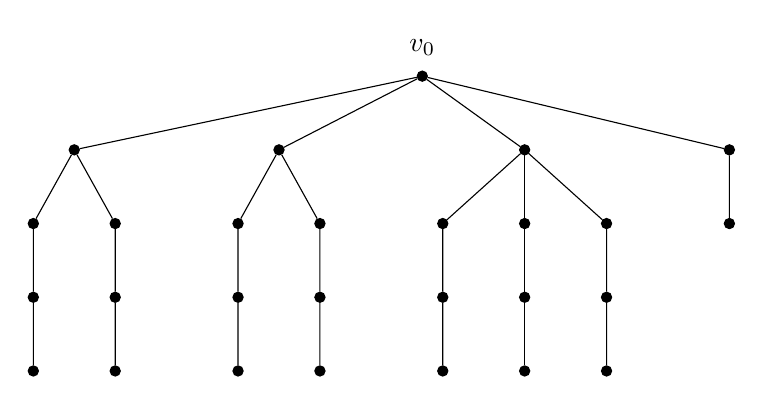
\begin{tikzpicture}[x=0.52cm,y=0.72cm,
  every node/.style={circle,draw,fill=black,inner sep=1.3pt}]
  \node (r) at (10.5,0) {};
  \node (h1) at (2,-1.3) {}; \node (h2) at (7,-1.3) {}; \node (h3) at (13,-1.3) {};
  \node (p1) at (18,-1.3) {}; \node (p2) at (18,-2.6) {};
  \draw (r)--(h1) (r)--(h2) (r)--(h3) (r)--(p1)--(p2);
  \foreach \h/\x in {h1/1,h1/3,h2/6,h2/8,h3/11,h3/13,h3/15}{
    \node (a) at (\x,-2.6) {}; \node (b) at (\x,-3.9) {}; \node (c) at (\x,-5.2) {};
    \draw (\h)--(a)--(b)--(c);
  }
  \node[draw=none,fill=none] at (10.5,0.5) {$v_0$};
\end{tikzpicture}
\caption{꼭짓점이 $27$개인 나무 $U$.}\label{fig:U}
\end{figure}

\begin{proposition}\label{prop:U}
나무 $U$는 $\gamma(U)=9$를 만족하고
\begin{align*}
 D(U,x)={}& 2x^{9}+75x^{10}+2837x^{11}+27278x^{12}+132791x^{13}+403364x^{14}\\
 &+842457x^{15}+1277429x^{16}+1454340x^{17}+1270263x^{18}+862444x^{19}\\
 &+458002x^{20}+190138x^{21}+61213x^{22}+15015x^{23}+2718x^{24}\\
 &+343x^{25}+27x^{26}+x^{27}
\end{align*}
이다. $d_{10}^2=5625<5674=d_{9}d_{11}$이므로 다항식 $D(U,x)$는 로그오목이 아니다.
이 다항식은 단봉이다.
\end{proposition}

\begin{proof}
다항식은 부록~\ref{app:computation}의 점화식 \eqref{eq:dp}로 계산하였고, $V(U)$의
부분집합 $2^{27}$개를 모두 나열하여 확인하였다.
\end{proof}

\begin{theorem}\label{thm:unique}
동형을 무시하면, 꼭짓점이 $27$개인 나무 가운데 지배다항식이 로그오목이 아닌 것은
$U$뿐이다.
\end{theorem}

\begin{proof}
이것 역시 부록~\ref{app:computation}에 기술한 전수 계산의 결과이며, 이 계산은 꼭짓점이
$27$개인 나무 $751\,065\,460$개를 모두 다룬다.
\end{proof}

\begin{proof}[정리~\ref{thm:smalltrees-intro}의 증명]
(i)은 정리~\ref{thm:small}과 따름정리~\ref{cor:smallforest}이고, (ii)는
명제~\ref{prop:U}와 정리~\ref{thm:unique}이다.
\end{proof}

\begin{remark}\label{rem:mechanism}
$U$에서 로그오목성이 깨지는 원인은 꼭짓점 $v_0$에서 찾을 수 있다. $v_0$을 포함하는
$U$의 지배집합은 $d_9$, $d_{10}$, $d_{11}$에 각각 $2$, $75$, $1141$만큼 기여하고, 이
세 수만 보면 $75^2\ge2\cdot1141$이 성립한다. $v_0$을 포함하지 않는 지배집합은 최소
지배집합보다 꼭짓점이 적어도 두 개 더 많다. 그러나 $v_0$의 이웃 $v_i$를 포함하는
순간, $v_i$에 매달린 $k_i$개의 경로 각각을 가운데 꼭짓점으로도 끝 꼭짓점으로도 지배할
수 있게 된다. $v_0$을 포함하지 않는 크기 $11$의 지배집합은 $1696$개이고,
$d_{11}=1141+1696=2837$은 $75^2/2$를 1퍼센트 미만의 차이로 넘는다. 꼭짓점이 $25$개인
나무 $T(2,2,3)$에서 같은 분해를 하면 $d_8=1$, $d_9=37$, $d_{10}=552+800=1352$를 얻는데,
이는 $37^2=1369$에 조금 못 미친다.
\end{remark}

\begin{remark}\label{rem:family}
$r\le5$이고 꼭짓점이 $34$개 이하인 나무 $T(k_1,\dots,k_r)$ 가운데 지배다항식이
로그오목이 아닌 것은 정확히 여섯 개이다. 위수 $28$의 $T(2,3,3)$, 위수 $31$의
$T(2,3,4)$와 $T(3,3,3)$, 위수 $34$의 $T(2,3,5)$, $T(2,4,4)$, $T(3,3,4)$이다. 이
나무들에서는 $U$에서와 마찬가지로 로그오목성이 첨수 $\gamma+1$에서만 깨지고, 다항식은
단봉이다. 특히 \cite[Proposition~1]{BS}에서 다루지 않은 나무 $T_3=T(3,3,3)$이 이미
로그오목이 아니다.
\end{remark}

\section{맺음말}\label{sec:remarks}

\subsection*{간격 5}
$h=5$일 때 정리~\ref{thm:criterion-intro}가 남기는 것은 고립점이 없고 꼭짓점이
$33$개 이하이며 $n-\gamma\le19$인 숲이다. 따름정리~\ref{cor:smallforest}에 의해, 이런
숲 가운데 지배다항식이 단봉이 아닌 것이 있다면 꼭짓점이 $\MinNonLC$개 이상인 성분을
가진다. 꼭짓점이 $33$개 이하인 나무를 모두 처리하는 것은 여기서 사용한 프로그램의
범위를 벗어나며, 명제~\ref{prop:U}는 이 범위에서 로그오목성을 더 이상 단봉성의
대용으로 쓸 수 없음을 보여 준다.

\begin{problem}
$\Gamma(F)-\gamma(F)=5$인 모든 숲 $F$의 지배다항식이 단봉임을 증명하라.
\end{problem}

\subsection*{도약의 크기}
정리~\ref{thm:main}의 증명은
\begin{equation}\label{eq:jumpquestion}
  c_{j+1}(G)-c_j(G)\le 2\qquad(\gamma(G)<j<n)
\end{equation}
가 성립하기만 하면 그래프 $G$의 지배다항식이 단봉임을 보여 준다. \eqref{eq:mean}에
의해 이것은 부등식 $(n-j+1)\,d_{j-1}d_{j+1}\le d_jd_{j+1}+(n-j)\,d_j^2$들과 같다.
보조정리~\ref{lem:jump}의 증명에서는 분산 $v_j$를 $a(S)$의 범위와 양립하는 가장 큰
값으로 평가하는데, 이 값은 두 극단값에 집중된 분포에서만 얻어질 수 있다. 이 거친
단계 때문에 결과가 $\sqrt n$ 크기의 간격으로 제한된다.

부등식 \eqref{eq:jumpquestion}은 꼭짓점이 $\MaxOrder$개 이하인 모든 나무에서 성립하며, 이
나무들 전체에서 $c_{j+1}-c_j$의 최댓값은 $\MaxJumpValue$보다 작다. 꼭짓점이 $34$개에서
$58$개인 나무에 대한 담금질 기법의 발견적 탐색에서도 $1.31$보다 큰 값은 나오지
않았다(보충자료). 그럼에도 이 부등식이 모든 나무에서 성립하는 것은 아니다.
$\gamma\le j\le n$에 대해
\[
  e_j=j-c_j=(n-j+1)\,\frac{d_{j-1}}{d_j}
\]
로 둔다. 이것은 크기 $j$인 지배집합에서 임계가 아닌 꼭짓점의 평균 개수이며,
$\gamma\le j<n$에서 $c_{j+1}-c_j=1+e_j-e_{j+1}$이다.

\begin{proposition}\label{prop:jumps}
\begin{enumerate}
\item[\textup{(i)}] $F$가 위수 $n$인 숲이고 $\gamma(F)<j<n$이면
$c_{j+1}-c_j<2\bigl(j-\gamma(F)\bigr)+1$이다.
\item[\textup{(ii)}] 모든 정수 $t\ge1$과 모든 $\varepsilon>0$에 대해, $j=\gamma(T)+t$에서
$c_{j+1}(T)-c_j(T)>2t+1-\varepsilon$인 나무 $T$가 존재한다.
\end{enumerate}
특히 \eqref{eq:jumpquestion}은 어떤 나무에서는 성립하지 않으며, 차 $c_{j+1}-c_j$는 나무
전체에서 유계가 아니다.
\end{proposition}

\begin{proof}
(i) 보조정리~\ref{lem:lower}에 의해 모든 $S\in\Dom_j(F)$에 대해
$j-a(S)\le2(j-\gamma)$이므로 $e_j\le2(j-\gamma)$이다. 또 $d_j>0$이고 $j<n$이므로
$e_{j+1}>0$이다.

(ii) $r=t+2\ge3$이라 하자. 정수 $k,M\ge1$에 대해, 성분이 $r$개인 $T(k,\dots,k)$의
$v_0$에 꼭짓점 두 개짜리 경로 $M$개를 각각 한 끝점으로 이어 붙인 나무를 $W$라 하자.
$W$의 위수는 $n=1+r+3rk+2M$이다. $W$의 뿌리를 $v_0$으로 잡고 \eqref{eq:dp}를 적용한다.
$v_i$에 붙은 꼭짓점 세 개짜리 경로는 $v_i$에 인접한 끝점에서
$(A+B+C,\;A+B,\;B)=\bigl(x(x+1)(x+2),\;x(x^2+3x+1),\;x(x+1)\bigr)$이고, $v_0$에 붙은
꼭짓점 두 개짜리 경로는 $(A+B+C,\;A+B,\;B)=\bigl(x(x+2),\;x(x+2),\;x\bigr)$이다.
\[
  f=x\bigl((x+1)(x+2)\bigr)^k+(x^2+3x+1)^k,\qquad g=f-(x+1)^k,\qquad
  w=(x^2+3x+1)^k-(x+1)^k
\]
로 두면 $1\le i\le r$에 대해 $A_{v_i}+B_{v_i}+C_{v_i}=x^kf$, $A_{v_i}+B_{v_i}=x^kg$,
$B_{v_i}=x^kw$이고, 따라서
\begin{equation}\label{eq:W}
  D(W,x)=x^{rk+M}\Bigl((x+2)^M\bigl(xf^r+g^r\bigr)-w^r\Bigr)
\end{equation}
이다. 여기서 $f(0)=1$이고, $g$와 $w$는 상수항이 $0$이며 일차 계수가 각각 $2^k+2k$와
$2k$이다. $\Phi=(x+2)^Mf^r$이라 하고 $x^s$의 계수를 $[x^s]\Phi$로 쓴다. $r\ge3$이므로
\eqref{eq:W}에서 $\gamma(W)=rk+M+1$이고
\begin{equation}\label{eq:Wlow}
  d_{\gamma+s}=[x^s]\Phi\quad(0\le s\le r-2),\qquad
  d_{\gamma+r-1}=[x^{r-1}]\Phi+2^M(2^k+2k)^r-(2k)^r\ \ge\ 2^{M+rk}
\end{equation}
이다. 계수별로 $(x+1)(x+2)\le2(1+x)^2$이고 $x^2+3x+1\le(1+2x)^2$이므로, $i\ge1$에 대해
$f$의 $x^i$ 계수는 $2^k\binom{2k}{i-1}+2^i\binom{2k}{i}\le2^k(4k)^i$ 이하이다. $f^r$을
전개할 때 $x$의 양의 거듭제곱을 내는 인수는 많아야 $\min(i,r)$개이므로, $1\le i\le r$에
대해 $[x^i]f^r\le2^{r+i}(4k)^i2^{ki}$이다. 이하에서는 $M>r-1$이라 가정한다. 아래에서 선택하는 $M$은 충분히 큰 $k$에 대해 이 조건을 만족한다. 그러므로 $0\le s\le r-1$에 대해
\[
  [x^s]\Phi=\sum_{i=0}^{s}[x^i]f^r\binom{M}{s-i}2^{M-s+i}
  =\binom Ms2^{M-s}\bigl(1+\theta_s\bigr),\qquad
  0\le\theta_s\le2^r\sum_{i=1}^{s}\Bigl(\frac{16\,k\,s\,2^k}{M-s}\Bigr)^{i}
\]
이다. 여기서 $\binom{M}{s-i}\big/\binom Ms\le\bigl(s/(M-s)\bigr)^i$을 썼다. 이제
$M=2^{k+\lceil k/(2r-2)\rceil}$로 두고 $k\to\infty$로 보내면 $k2^k/M\to0$이고
$M^{r-1}/2^{rk}\to0$이므로, 각 $s\le r-1$에 대해 $\theta_s\to0$이다. $t=r-2$,
$j=\gamma+t$라 하자. $n-\gamma=M+2rk+r$이므로 \eqref{eq:Wlow}에 의해
\[
  e_j=(n-j+1)\frac{d_{\gamma+t-1}}{d_{\gamma+t}}
     =(M+2rk+r-t+1)\,\frac{2t}{M-t+1}\cdot\frac{1+\theta_{t-1}}{1+\theta_t}
     \longrightarrow2t ,
\]
\[
  e_{j+1}=(n-j)\frac{d_{\gamma+t}}{d_{\gamma+t+1}}
     \le(M+2rk+r)\,\frac{M^{t}\,2^{M-t}(1+\theta_t)}{2^{M+rk}}
     \longrightarrow0
\]
이다. 따라서 $c_{j+1}-c_j=1+e_j-e_{j+1}\to2t+1$이다.
\end{proof}

$t=1$일 때 이 명제는 모든 숲에서 $c_{\gamma+2}-c_{\gamma+1}<3$이며 상수 $3$을 더 작은
수로 바꿀 수 없음을 말한다. $s\le r-2$일 때 $W$의 크기 $\gamma+s$인 지배집합은, 무시할
수 있는 비율을 제외하면, 최소 지배집합에 $v_0$에 붙은 경로 위의 꼭짓점 $s$개를 더한
것이고, 더한 꼭짓점 하나마다 두 꼭짓점이 임계가 아니게 된다. 반면 크기 $\gamma+r-1$인
지배집합은 $v_0$을 포함하지 않는 것이 압도적으로 많고 이들은 극소이다. 구체적으로,
$T(8,8,9)$의 $v_0$에 꼭짓점 두 개짜리 경로 $3211$개를 붙인 나무는 꼭짓점이 $6501$개이고
$c_{\gamma+2}-c_{\gamma+1}>2$를 만족한다. 또 $r=3$, $k=9$, $M=7700$인 나무 $W$는
꼭짓점이 $15\,485$개이고 $c_{\gamma+2}-c_{\gamma+1}>2.15$이다. 두 나무 모두
\eqref{eq:W}를 쓰지 않고 \eqref{eq:dp}로 지배다항식 전체를 계산하였다. 지배다항식은
단봉이며, \eqref{eq:jumpquestion}은 $j=\gamma+1$에서만 깨진다(보충자료). 같은
조각으로 만든 나무가 \cite{DHP}에서 다른 목적으로 쓰인다. 그 논문에서는 새 꼭짓점을
$T(k,k,k)$의 복사본 $m$개 각각의 $v_0$과, 꼭짓점 두 개짜리 경로의 한 끝 꼭짓점에
이으며, $k$가 크면 지표 $\gamma+1,\gamma+3,\dots,\gamma+2m-1$에서 로그오목성이
깨진다.

정리~\ref{thm:main}의 증명은 \eqref{eq:jumpquestion}을
따름정리~\ref{cor:segments}(i)의 증가 구간을 지난 지표에서만 사용하는 반면,
명제~\ref{prop:jumps}의 큰 도약은 $\gamma$ 바로 다음에서 일어난다. 이로부터 다음의 더
약한 질문이 나온다.

\begin{question}\label{q:jump}
$T$가 위수 $n$인 나무일 때, $(n+2\gamma(T)+1)/3<j<n$인 모든 $j$에 대해
$c_{j+1}(T)-c_j(T)\le2$인가?
\end{question}

답이 긍정이라면 정리~\ref{thm:main}의 증명에 의해 나무에 대한 단봉성 추측이 따라
나온다. 꼭짓점이 $26$개 이하인 모든 나무와 위에서 언급한 나무 $W$들에서는 이 범위의 차
$c_{j+1}-c_j$가 실제로 $1$보다 작다(보충자료).

이 범위의 위쪽 끝에서는 답이 긍정이다. $T$를 위수 $n\ge5$이고 잎이 $L$개인 나무라 하자.
이때 $\gamma(T)\le n/2<n-2$이다. 분명히 $c_n-c_{n-1}=-c_{n-1}\le0$이고, 나아가
\begin{equation}\label{eq:top}
  c_{n-1}-c_{n-2}\le1-\frac2n
\end{equation}
이 성립하며 등호는 $T$가 별일 때에만 성립한다. 꼭짓점 집합이 지배집합일 필요충분조건은 그
여집합이 어떤 닫힌 근방도 포함하지 않는 것이다. 원소가 두 개인 닫힌 근방은 잎의 닫힌
근방이고 이들은 서로 다르므로 $d_{n-2}=\binom n2-L$이다. 이들 각각은 꼭짓점 세 개로 된
집합 $n-2$개에 포함되고, 꼭짓점 세 개로 된 집합은 이들을 많아야 두 개 포함하며, 두 개를
포함하는 것은 두 잎의 이웃이 같을 때뿐이다. 따라서 닫힌 근방을 포함하는 세 꼭짓점
집합은 적어도 $L(n-2)-\binom L2$개이고, $u=\binom n3-L(n-2)+\binom L2$라 하면
$d_{n-3}\le u$이다. $b=d_{n-2}$라 하자. $d_{n-1}=n$이므로 \eqref{eq:mean}에 의해
$e_{n-1}=2b/n$, $e_{n-2}=3d_{n-3}/b$이고, 따라서 \eqref{eq:top}은
$3n\,d_{n-3}\le2b(b-1)$과 동치이다. 그런데 $L\le n-1$이므로
\[
  2b(b-1)-3nu=\tfrac12\,(n-1-L)\bigl(L(3n-4)+n(n-2)\bigr)\ge0
\]
이다. 우변이 $0$이 되는 것은 $L=n-1$, 즉 별 $K_{1,n-1}$일 때뿐이며, 이때
$d_{n-3}=u$이다.

\subsection*{숲 너머}
정리~\ref{thm:main}은 $(\mathrm{H}_h)$를 만족하는 모든 그래프에 적용된다.
보조정리~\ref{lem:upper}와 \eqref{eq:alpha-Gamma}에 의해 \eqref{eq:H}의 상계는 모든
이분그래프 $G$에서 $h=\Gamma(G)-\gamma(G)$로 성립하므로, 숲에 특유한 것은 하계
$a(S)\ge2\gamma(G)-|S|$뿐이다. 이 하계는 $C_4$에서 성립하지 않지만, 어떤 이분그래프에서
성립하는지 기술하는 것은 흥미로운 문제이다.

\subsection*{AI 도구 사용}
이 연구에서는 증명 탐색, 계산 프로그램과 Lean 코드 작성, 본문 초안 작성에 대규모 언어
모델 기반 AI 도구를 사용하였다. 저자는 모든 논증을 확인하였으며 그 내용에 대한 책임을
진다.

\subsection*{보충자료}
부록~\ref{app:computation}의 두 프로그램 소스 코드와 전체 출력, 본문에서 언급한 보조
스크립트, 부록~\ref{app:lean}의 Lean~4 소스는 저자에게서 얻을 수 있으며 원고와 함께
제출한다.

\appendix
\section{계산}\label{app:computation}

이 부록에서는 정리~\ref{thm:small}과 정리~\ref{thm:unique}의 바탕이 되는 계산을
기술한다. 모든 산술은 정확한 정수 산술이며, 보고하는 검사 어디에도 부동소수점 비교는
들어가지 않는다.

\subsection*{점화식}
$T$를 꼭짓점 $\rho$를 뿌리로 하는 나무라 하고, 꼭짓점 $v$에 대해 $v$와 그 자손이
유도하는 부분나무를 $T_v$라 하자. $V(T_v)$의 부분집합 $S$ 가운데, $v$가 아닌 $T_v$의
모든 꼭짓점이 $S$에 속하거나 $S$ 안에 이웃을 가지는 것을 생각한다. 이런 집합 중에서
각각 $v\in S$인 것, $v\notin S$이고 $v$의 어떤 자식이 $S$에 속하는 것, $v\notin S$이고
$v$의 어떤 자식도 $S$에 속하지 않는 것의 크기에 대한 생성 다항식을 $A_v$, $B_v$,
$C_v$라 하자. $v$가 잎이면 $(A_v,B_v,C_v)=(x,0,1)$이고, 그렇지 않으면 $w$가 $v$의
자식을 움직일 때
\begin{equation}\label{eq:dp}
  A_v=x\prod_w(A_w+B_w+C_w),\qquad
  B_v=\prod_w(A_w+B_w)-\prod_w B_w,\qquad
  C_v=\prod_w B_w
\end{equation}
이다. 실제로 $v\in S$이면 자식에는 제약이 없다. $v\notin S$이면 모든 자식이 자기
부분나무 안에서 지배되어야 하고, $C_v$는 어떤 자식도 선택되지 않은 집합을 모은다.
뿌리는 지배되어야 하므로 $D(T,x)=A_\rho+B_\rho$이다.

\subsection*{두 프로그램}
계산은 서로 독립적으로 작성한 프로그램으로 두 번 수행하였다.

\textbf{프로그램 I}은 Beyer와 Hedetniemi의 알고리즘~\cite{BH}으로 위수 $n$인 뿌리 있는
나무를 모두 수준 수열로 생성하고, 그 수가 고전적인 점화식
$(n-1)r_n=\sum_{j=1}^{n-1}\bigl(\sum_{d\mid j}d\,r_d\bigr)r_{n-j}$로 주어지는 뿌리 있는
나무의 수 $r_n$과 같은지 검사한다. 뿌리가 무게중심인 것만 남기고, 나무에 무게중심이
둘이면 두 뿌리 선택을 표준 부호로 비교하여 하나만 남긴다. 따라서 모든 나무가 정확히
한 번 처리되며, 프로그램은 처리한 나무의 수가 Otter의 공식~\cite{Otter}
\[
  t_n=r_n-\tfrac12\Bigl(\sum_{k=1}^{n-1}r_kr_{n-k}-[\,n\text{ 짝수}\,]\,r_{n/2}\Bigr)
\]
으로 주어지는 위수 $n$인 나무의 수와 같은지 검사한다. 지배다항식은 꼭짓점의 자식을
하나씩 병합하여 계산한다. 이것은 \eqref{eq:dp}와 동치인 형태
$(A,B,C)\mapsto\bigl(A(A_w+B_w+C_w),\,B(A_w+B_w)+CA_w,\,CB_w\bigr)$를 $(x,0,1)$에서
시작하여 적용하는 것이다. 위수 $16$ 이하의 모든 나무에 대해서는 꼭짓점 부분집합을 모두
나열하여, 그 결과로 얻은 지배집합의 수와 $\gamma$, $\Gamma$의 값을 점화식에서 얻은
값과 비교하고(프로그램은 $\Gamma$를 독립수로 계산한다. \eqref{eq:alpha-Gamma} 참조),
모든 지배집합에 대해 두 부등식 \eqref{eq:twosided}를 검사한다. 그런 나무는
$32\,507$개이고 불일치는 없다.

\textbf{프로그램 II}는 Wright, Richmond, Odlyzko, McKay의 알고리즘~\cite{WROM}으로 위수
$n$인 나무를 직접 생성하고, 그 수를 $t_n$과 대조하며, \eqref{eq:dp}를 적힌 그대로
계산한다.

두 프로그램 모두 $1\le j\le n-1$인 모든 $j$에 대해 $d_j^2\ge d_{j-1}d_{j+1}$을 128비트
정수 곱으로 검사한다. 고려하는 범위에서 계수 자체는 $2^{27}$보다 작다. 두 프로그램은
또한 위수마다, 그 위수의 모든 나무에 대한 계수 벡터의 64비트 해시의 합을 $2^{64}$를
법으로 하여 출력한다. 이 합은 $2$부터 $\MaxOrder$까지 모든 위수에서 일치한다. 이는
두 프로그램이 나무를 다른 순서로, 다른 뿌리로 순회하면서도 (해시 충돌을 제외하면) 같은
다항식 다중집합을 계산하였음을 보여 준다.

\subsection*{결과}
표~\ref{tab:counts}에 나무의 수를 싣는다. 지배다항식이 $x$인 꼭짓점 한 개짜리 나무를
더하면 꼭짓점이 $\MaxOrder$개 이하인 나무는 모두 $\TotalTreesAll$개이다. 두 프로그램 모두 꼭짓점이 $\MaxLC$개 이하인 모든
나무의 지배다항식이 로그오목이고, 꼭짓점이 $\MinNonLC$개인 나무 가운데 정확히 하나,
즉 그림~\ref{fig:U}의 나무 $U$만 이 성질을 가지지 않는다고 보고한다. 두 프로그램은
또한 이 지배다항식들이 모두 단봉이라고 보고한다.

\begin{table}[ht]
\centering
\caption{프로그램 I이 생성한 뿌리 있는 나무의 수 $r_n$과 두 프로그램이 조사한 나무의
수 $t_n$.}\label{tab:counts}
\smallskip
\begin{tabular}{rrr@{\qquad\qquad}rrr}
\hline
$n$ & $r_n$ & $t_n$ & $n$ & $r_n$ & $t_n$\\
\hline
2 & 1 & 1 & 15 & 87\,811 & 7\,741\\
3 & 2 & 1 & 16 & 235\,381 & 19\,320\\
4 & 4 & 2 & 17 & 634\,847 & 48\,629\\
5 & 9 & 3 & 18 & 1\,721\,159 & 123\,867\\
6 & 20 & 6 & 19 & 4\,688\,676 & 317\,955\\
7 & 48 & 11 & 20 & 12\,826\,228 & 823\,065\\
8 & 115 & 23 & 21 & 35\,221\,832 & 2\,144\,505\\
9 & 286 & 47 & 22 & 97\,055\,181 & 5\,623\,756\\
10 & 719 & 106 & 23 & 268\,282\,855 & 14\,828\,074\\
11 & 1\,842 & 235 & 24 & 743\,724\,984 & 39\,299\,897\\
12 & 4\,766 & 551 & 25 & 2\,067\,174\,645 & 104\,636\,890\\
13 & 12\,486 & 1\,301 & 26 & 5\,759\,636\,510 & 279\,793\,450\\
14 & 32\,973 & 3\,159 & 27 & 16\,083\,734\,329 & 751\,065\,460\\
\hline
\end{tabular}

\end{table}

두 프로그램의 소스 코드, 전체 출력, 비고~\ref{rem:boundary}의 수를 다시 계산하는
스크립트, 주어진 나무의 모든 부분집합을 나열하는 프로그램(명제~\ref{prop:U}에 사용)은
보충자료에 들어 있다.

\section{형식 검증}\label{app:lean}

다음 명제들은 Mathlib을 사용하는 Lean~4(버전 4.27.0)~\cite{Lean,Mathlib}로 형식화하고
검사하였다. 형식 전개에서 그래프는 유한 꼭짓점 유형 위의 Mathlib 유형
\texttt{SimpleGraph}의 항이고, 숲은 사이클이 없는 그래프이며, $\gamma$와 $\Gamma$는
정의된 불변량이 아니라 명시적인 증인과 부등식으로 규정한다. 예를 들어 $\gamma$는
어떤 지배집합의 원소가 $\gamma$개 이하이고 모든 지배집합의 원소가 $\gamma$개 이상인
자연수이다.

\begin{itemize}
\item 보조정리~\ref{lem:lower}
(\lean{forest_critical_inequality})와 보조정리~\ref{lem:upper}
(\lean{bipartite_critical_le_two_independence}).
\item 정리~\ref{thm:main}의 핵심
(\lean{graph_uniform_gap_unimodal}): 유한 유형 위의 임의의 관계, $(h+1)^2\le4K$인
자연수 $h<K$, 그리고 $\gamma+K\le A+2\le n$이며 거기까지 계수가 감소하지 않는 첨수
$A$에 대해, 조건 $(\mathrm{H}_h)$는 단봉성을 함의한다.
\item 고립점이 없고 간격이 정확히 3인 숲에 대한 따름정리~\ref{cor:gapthree}
(\lean{forest_gap_three_unimodal_no_isolates}).
\item $h=4$에 대한 정리~\ref{thm:criterion-intro}(i)
(\lean{forest_gap_four_large_unimodal}), 그리고 고립점이 없고 크기 $\gamma+4$인 극소
지배집합을 가지는 그래프는 $n\ge\gamma+14$ 또는 $n\le22$를 만족한다는 사실
(\lean{no_isolates_gap_four_large_or_at_most_twenty_two}).
\end{itemize}

이 정리들은 모두 Lean의 고전 논리의 표준 공리 세 개(\lean{propext},
\texttt{Classical.choice}, \texttt{Quot.sound})에만 의존한다. 형식화는 고립점이 없는
숲으로의 환원(보조정리~\ref{lem:isolates}), 여기서 제시한 형태의 일반적인 $h$에 대한
정리~\ref{thm:criterion-intro}, 보조정리~\ref{lem:product}, 그리고
부록~\ref{app:computation}의 계산의 어떤 부분도 포함하지 \textbf{않는다}. 특히
정리~\ref{thm:small}과 정리~\ref{thm:unique}, 그리고 전자에 의존하는
정리~\ref{thm:gapfour-intro}의 간격 4인 경우는 통상적인 의미의 컴퓨터 보조 결과이며
형식적으로 검증된 결과가 아니다. Lean 소스는 보충자료에 들어 있다.

\begin{thebibliography}{99}

\bibitem{AP} S. Alikhani and Y.-H. Peng,
{\it Introduction to domination polynomial of a graph},
Ars Combin. {\bf 114} (2014), 257--266.

\bibitem{BB21} I. Beaton and J. I. Brown,
{\it The average order of dominating sets of a graph},
Discrete Math. {\bf 344} (12) (2021), 112595.
\\ {\tiny \url{https://doi.org/10.1016/j.disc.2021.112595} }

\bibitem{BB22} I. Beaton and J. I. Brown,
{\it On the unimodality of domination polynomials},
Graphs Combin. {\bf 38} (3) (2022), 90.
\\ {\tiny \url{https://doi.org/10.1007/s00373-022-02487-x} }

\bibitem{BS} I. Beaton and S. Schoonhoven,
{\it On the unimodality of nearly well-dominated trees},
preprint, arXiv:2411.02288 (2024).
\\ {\tiny \url{https://arxiv.org/abs/2411.02288} }

\bibitem{BH} T. Beyer and S. M. Hedetniemi,
{\it Constant time generation of rooted trees},
SIAM J. Comput. {\bf 9} (4) (1980), 706--712.
\\ {\tiny \url{https://doi.org/10.1137/0209055} }

\bibitem{BO} A. Burcroff and G. O'Brien,
{\it Unimodality and monotonic portions of certain domination polynomials},
Discrete Math. {\bf 346} (9) (2023), 113508.
\\ {\tiny \url{https://doi.org/10.1016/j.disc.2023.113508} }

\bibitem{CFPT} E. J. Cockayne, O. Favaron, C. Payan and A. G. Thomason,
{\it Contributions to the theory of domination, independence and irredundance in graphs},
Discrete Math. {\bf 33} (3) (1981), 249--258.
\\ {\tiny \url{https://doi.org/10.1016/0012-365X(81)90268-5} }

\bibitem{Lean} L. de Moura and S. Ullrich,
{\it The Lean 4 theorem prover and programming language},
in: Automated Deduction -- CADE 28, Lecture Notes in Comput. Sci. 12699, Springer, Cham, 2021, pp.~625--635.
\\ {\tiny \url{https://doi.org/10.1007/978-3-030-79876-5_37} }

\bibitem{DHP} A. Du, S. Heilman and G. Panova,
{\it Trees and graphs with non log-concave dominating set sequence via AI tools},
preprint, arXiv:2605.02193 (2026).
\\ {\tiny \url{https://arxiv.org/abs/2605.02193} }

\bibitem{GZ} D. Galvin and Y. Zhang,
{\it The domination polynomial of powers of paths and cycles},
preprint, arXiv:2408.12731 (2024).
\\ {\tiny \url{https://arxiv.org/abs/2408.12731} }

\bibitem{KL} O. Kadrawi and V. E. Levit,
{\it The independence polynomial of trees is not always log-concave starting from order 26},
Ars Math. Contemp. {\bf 25} (4) (2025), \#P4.03.
\\ {\tiny \url{https://doi.org/10.26493/1855-3974.3207.2ad} }

\bibitem{Mathlib} The mathlib Community,
{\it The Lean mathematical library},
in: Proceedings of the 9th ACM SIGPLAN International Conference on Certified Programs and Proofs (CPP 2020), ACM, New York, 2020, pp.~367--381.
\\ {\tiny \url{https://doi.org/10.1145/3372885.3373824} }

\bibitem{Omar} M. Omar,
{\it New perspectives on the unimodality of domination polynomials},
preprint, arXiv:2601.14494 (2026).
\\ {\tiny \url{https://arxiv.org/abs/2601.14494} }

\bibitem{Ore} O. Ore,
{\it Theory of Graphs},
Amer. Math. Soc. Colloq. Publ. 38, American Mathematical Society, Providence, RI, 1962.

\bibitem{Otter} R. Otter,
{\it The number of trees},
Ann. of Math. (2) {\bf 49} (3) (1948), 583--599.
\\ {\tiny \url{https://doi.org/10.2307/1969046} }

\bibitem{Stanley} R. P. Stanley,
{\it Log-concave and unimodal sequences in algebra, combinatorics, and geometry},
Ann. New York Acad. Sci. {\bf 576} (1989), 500--535.
\\ {\tiny \url{https://doi.org/10.1111/j.1749-6632.1989.tb16434.x} }

\bibitem{WROM} R. A. Wright, B. Richmond, A. Odlyzko and B. D. McKay,
{\it Constant time generation of free trees},
SIAM J. Comput. {\bf 15} (2) (1986), 540--548.
\\ {\tiny \url{https://doi.org/10.1137/0215039} }

\end{thebibliography}


\end{document}

